\section{Results}

\begin{frame}
    \frametitle{AE-(dp)MERF}

    \begin{columns}
        \begin{column}{0.48\textwidth}
        \begin{figure}
            \centering
            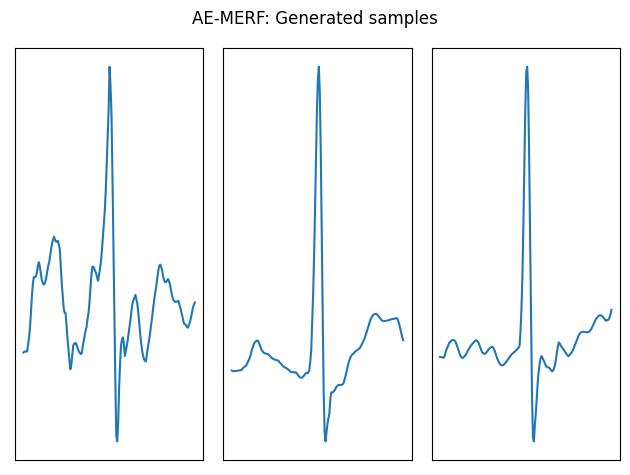
\includegraphics[scale=0.25]{gen_aemerf.png}
        \end{figure}
        \begin{figure}[h]
            \centering
            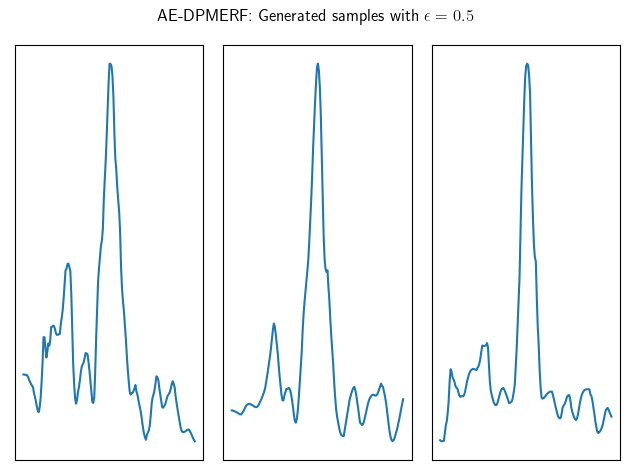
\includegraphics[scale=0.25]{gen_aedpmerf_eps05.png}
        \end{figure}
    \end{column}
    \begin{column}{0.48\textwidth}
        \begin{figure}
            \centering
            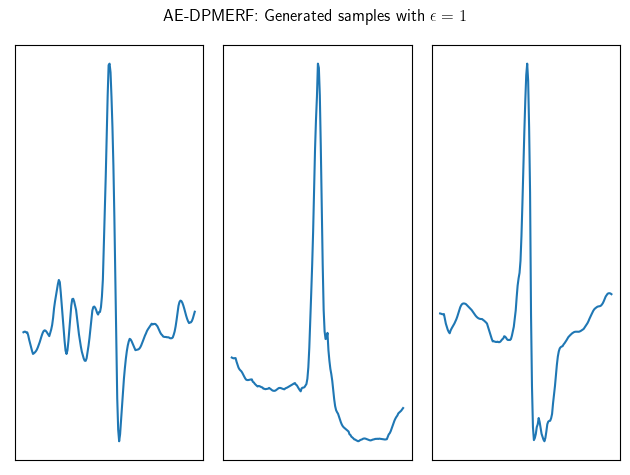
\includegraphics[scale=0.25]{gen_aedpmerf_eps1.png}
        \end{figure}
        \begin{figure}[h]
            \centering
            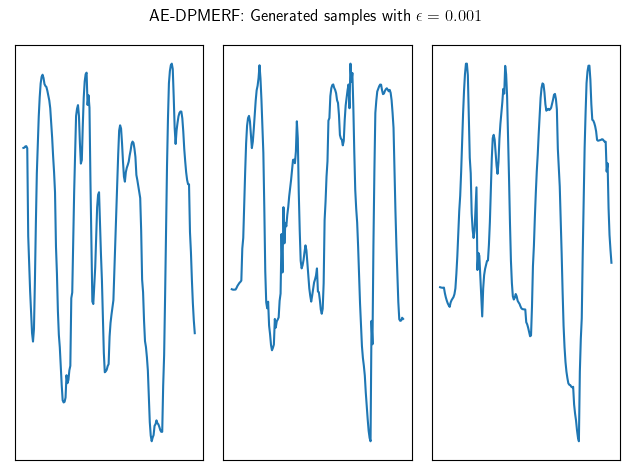
\includegraphics[scale=0.25]{gen_aedpmerf_eps001.png}
        \end{figure}
    \end{column}
    
    \end{columns}
    \centering
    \textcolor{gold}{Figure:} AE-(dp)MERF generated samples

\end{frame}

\begin{frame}{AE-(DP)MERF}
    \begin{figure}
        \centering
        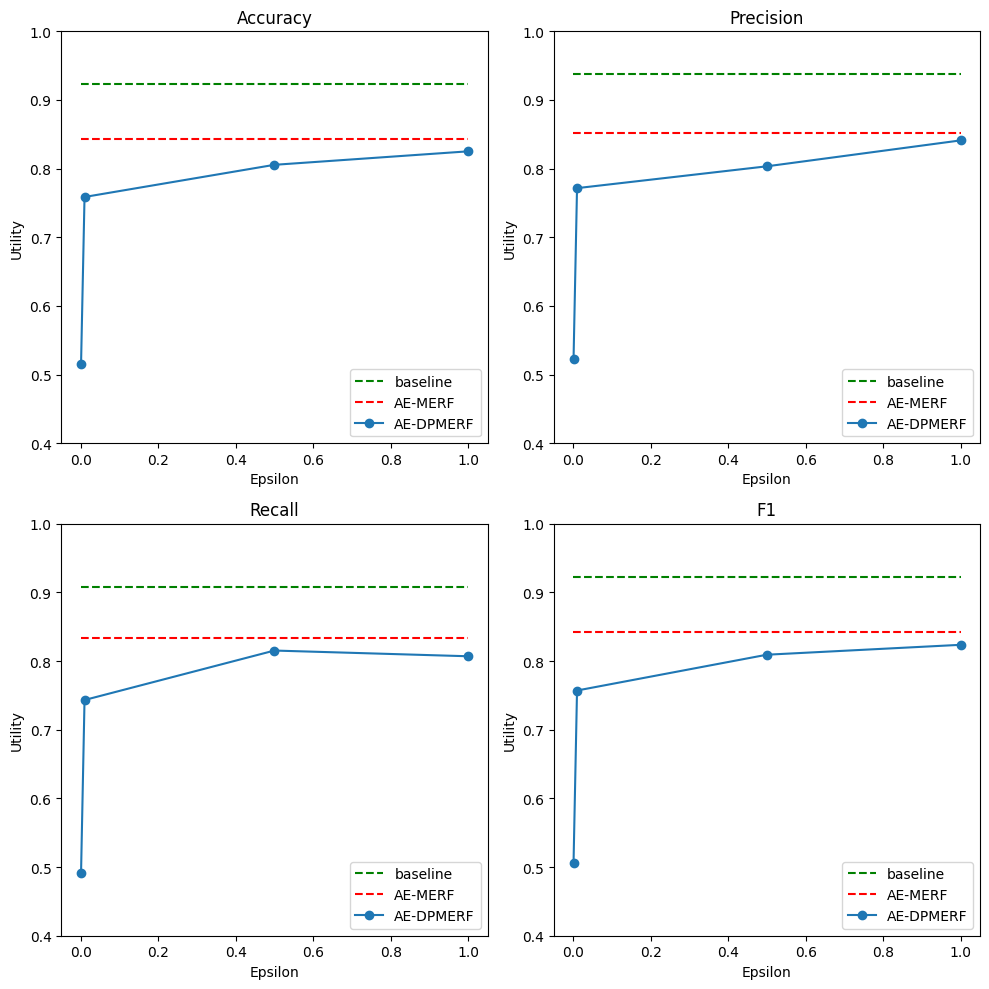
\includegraphics[scale=0.23]{results_aedpmerf.png}
        \caption{Results of AE-(DP)MERF with different privacy budgets (lower epsilon means higher privacy)}
        \label{fig:enter-label}
    \end{figure}
\end{frame}

\begin{frame}
    \frametitle{AE-(dp)WGAN}

    \begin{columns}
        \begin{column}{0.48\textwidth}
        \begin{figure}
            \centering
            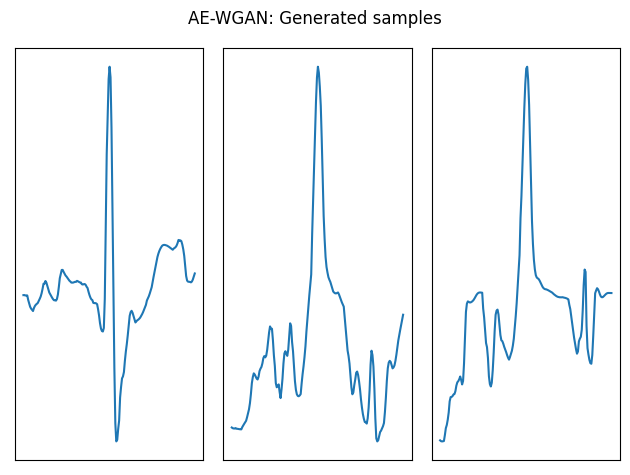
\includegraphics[scale=0.25]{gen_aewgan.png}
        \end{figure}
        \begin{figure}[h]
            \centering
            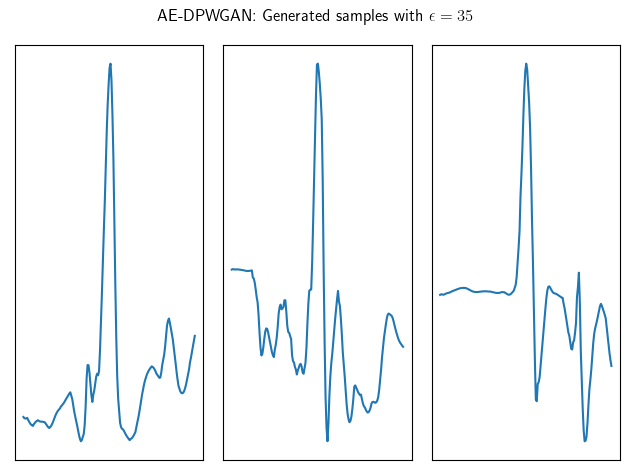
\includegraphics[scale=0.25]{gen_aedpwgan_eps35.png}
        \end{figure}
    \end{column}
    \begin{column}{0.48\textwidth}
        \begin{figure}
            \centering
            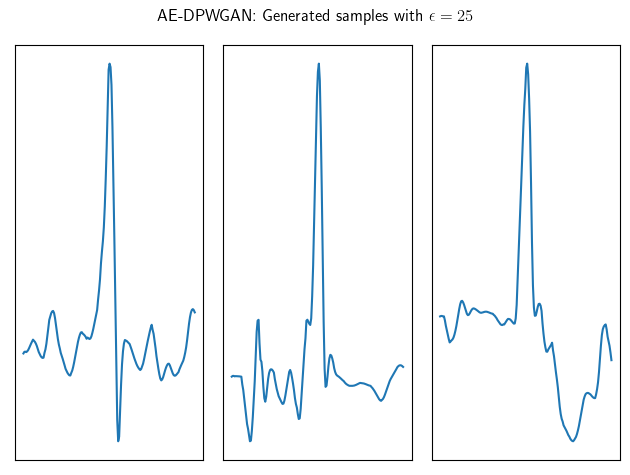
\includegraphics[scale=0.25]{gen_aedpwgan_eps25.png}
        \end{figure}
        \begin{figure}[h]
            \centering
            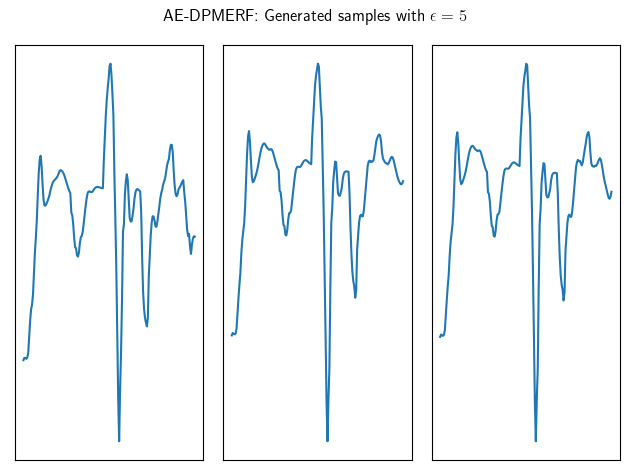
\includegraphics[scale=0.25]{gen_aedpwgan_eps5.png}
        \end{figure}
    \end{column}
    
    \end{columns}
    \centering
    \textcolor{gold}{Figure:} AE-(dp)WGAN generated samples

\end{frame}

\begin{frame}{AE-(dp)WGAN}
    \begin{figure}
        \centering
        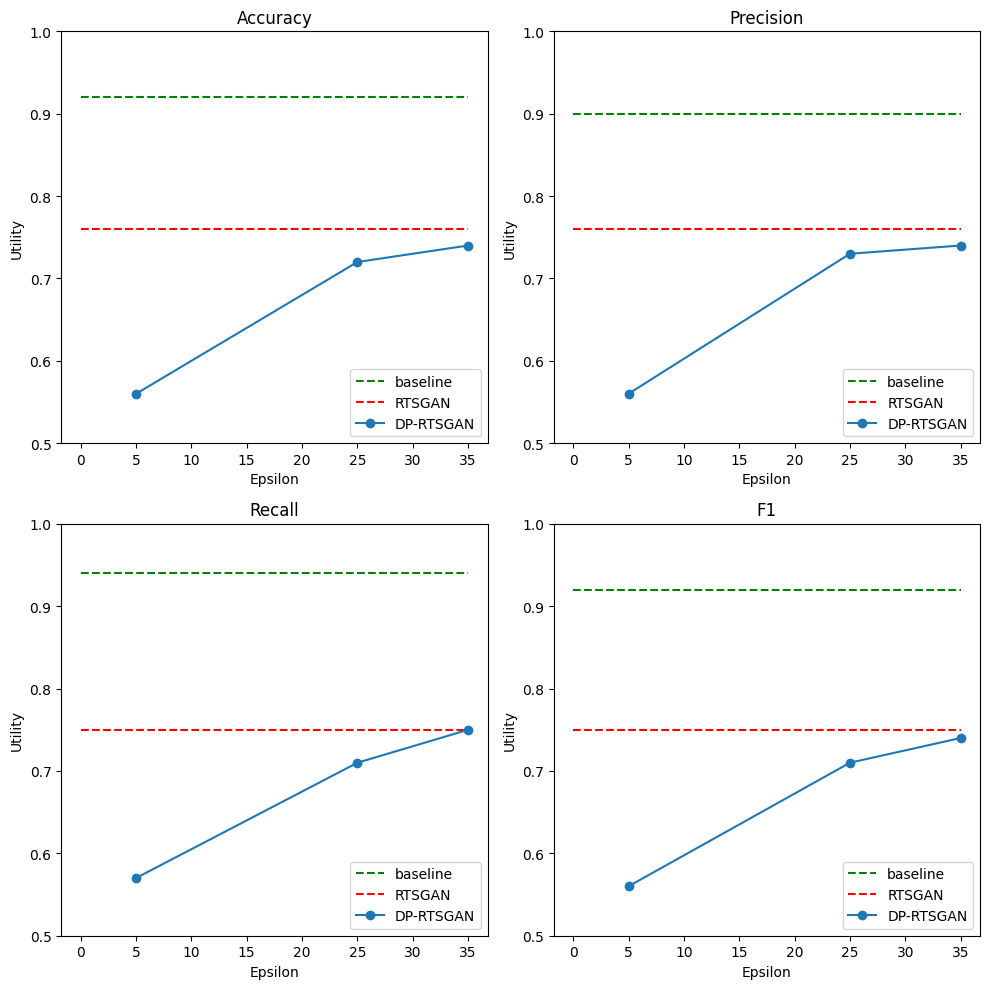
\includegraphics[scale=0.23]{restuls_dprtsgan.png}
        \caption{Results of AE-(dp)WGAN with different privacy budgets (lower epsilon means higher privacy)}
        \label{fig:enter-label}
    \end{figure}
\end{frame}

\begin{frame}{Conclusion}
    \begin{itemize}
        \item<1-> \alert{AE-(dp)MERF performs best} and is very efficient computationally.
        \item<2-> AE-(dp)MERF can work in \alert{lower epsilon ranges}, which translates to \alert{stronger privacy guarantees}.
        \item<3-> \alert{AE-(dp)WGAN gives worse utility} and can only work with meaningless privacy budgets $\epsilon$.
        \item<4-> We lose utility when \alert{replacing original data with non-private synthetic} data.
        \item<5-> BUT: Adding \alert{privacy does not further degrade the utility} for anomaly detection too much until too much noise is added.
    \end{itemize}
\end{frame}

\begin{frame}{Contamination}
    We \alert{contaminate} the train set that only consists of regular samples with \alert{1\%, 2\%, 5\% anomalous samples} (the percentage of heartbeat arrhythmias is estimated to be around max. 5\%).
\end{frame}

\begin{frame}{Contamination}

    \begin{figure}[h]
        \centering
        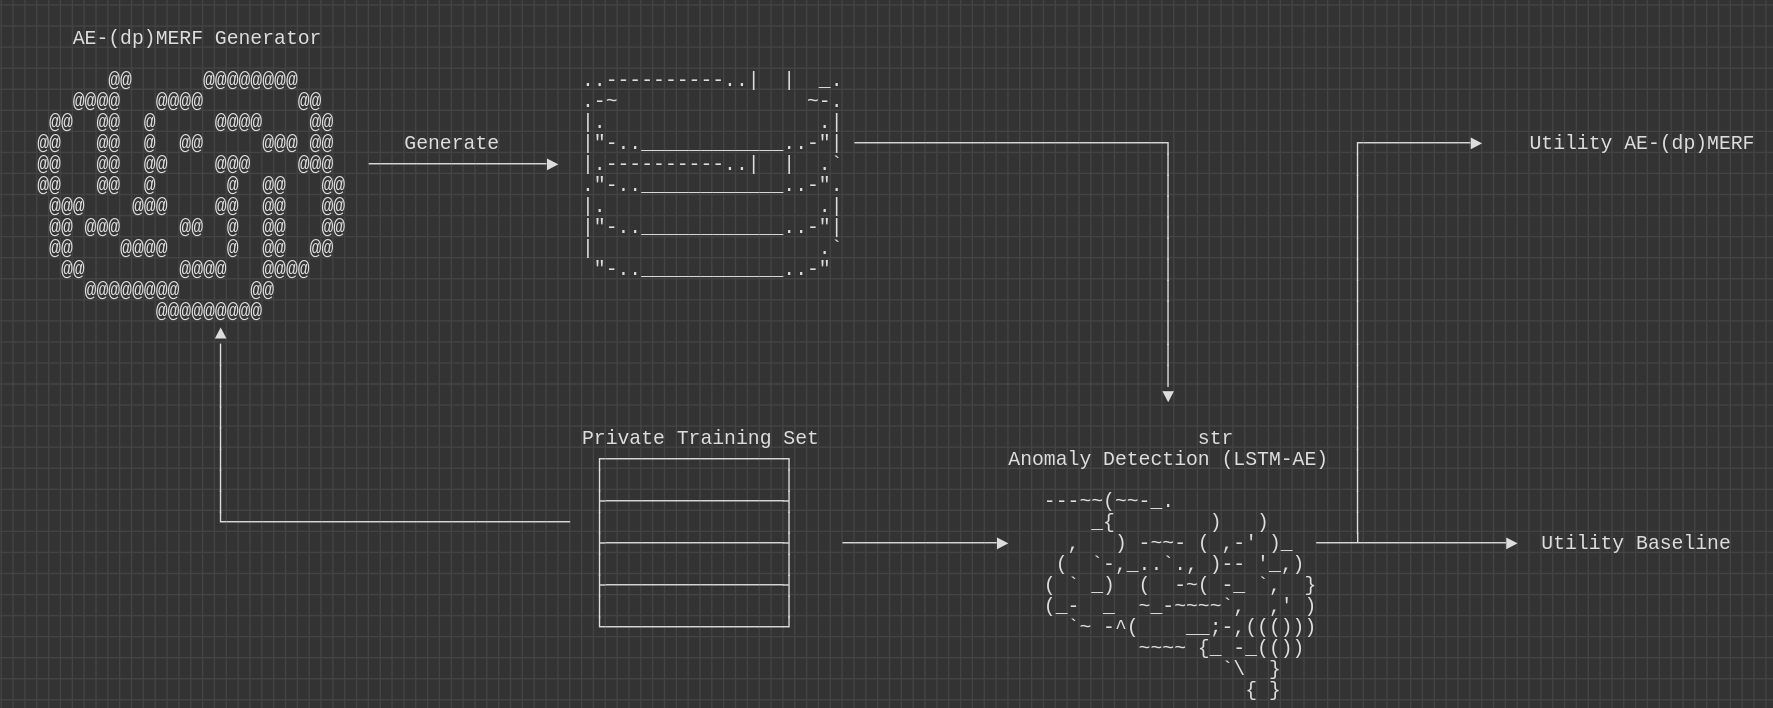
\includegraphics[scale=0.28]{str_comtam.png}
        \caption{Structure of Contamination Experiment}
        \label{fig:enter-label}
    \end{figure}

\end{frame}

\begin{frame}{Contamination: AE-(DP)MERF}
    \begin{figure}

        \centering
        \only<1>{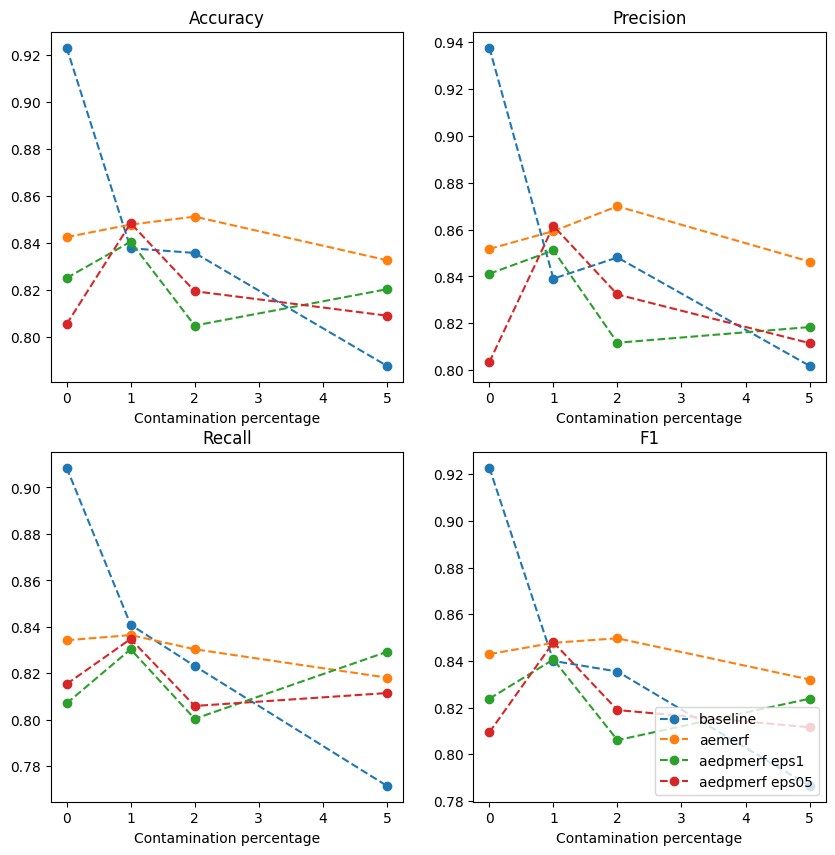
\includegraphics[width=0.8\textheight]{results_aedpmerf_contam.png}}%
        \only<2>{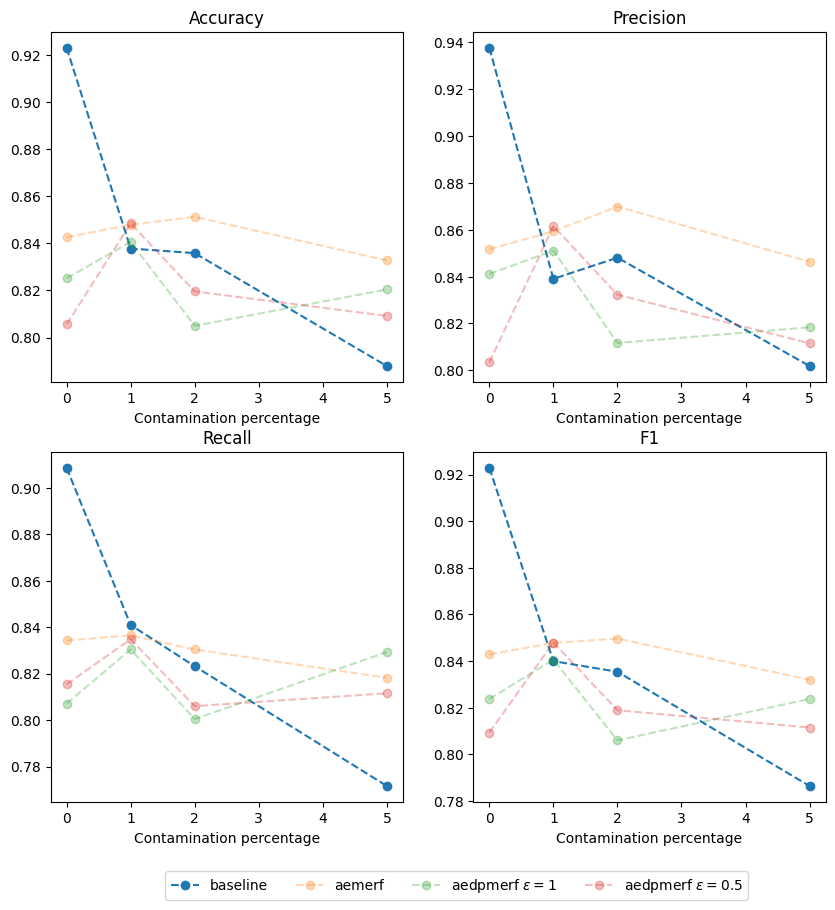
\includegraphics[width=0.8\textheight]{results_aedpmerf_contam_baseline.png}}%
        \only<3>{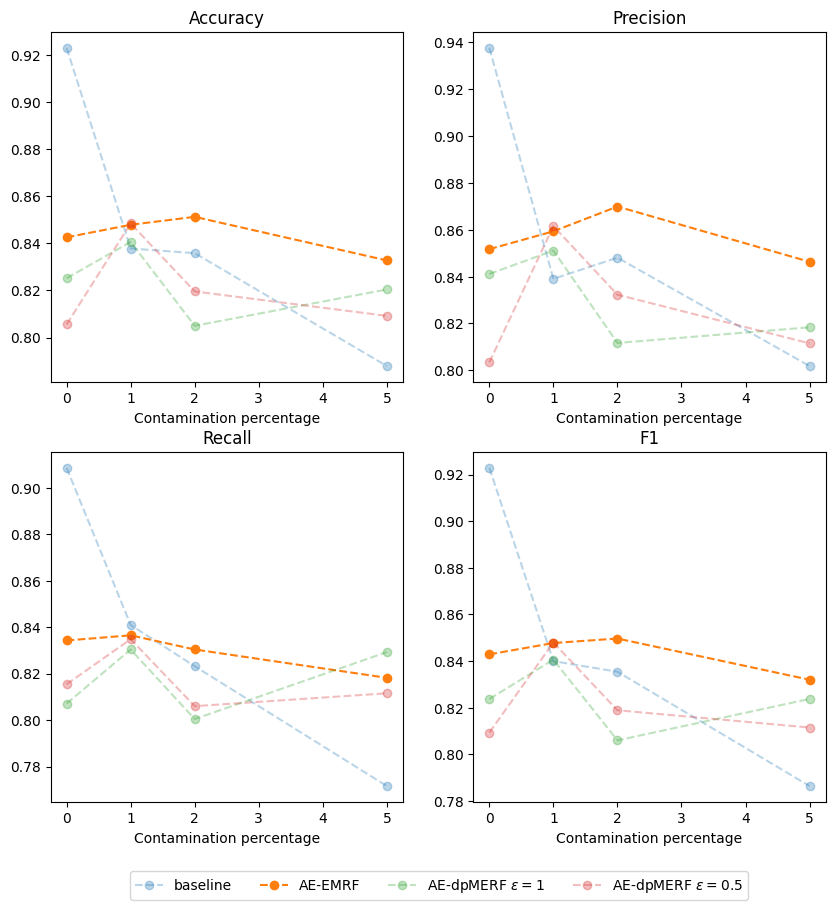
\includegraphics[width=0.8\textheight]{results_aedpmerf_contam_aemerf.png}}%
        \only<4>{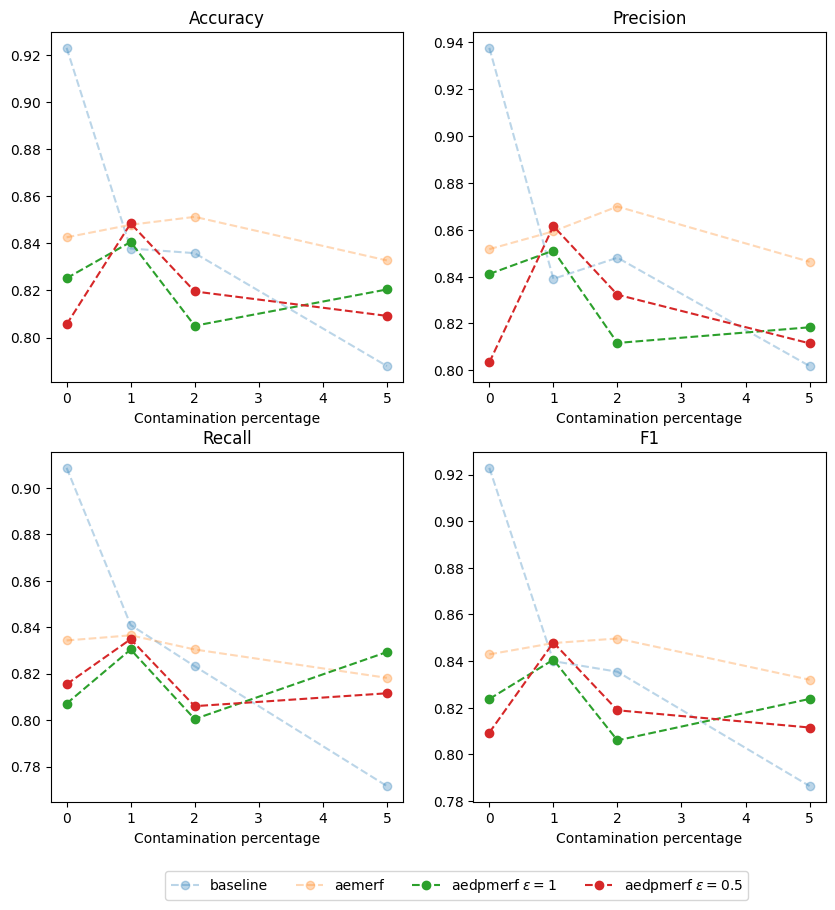
\includegraphics[width=0.8\textheight]{results_aedpmerf_contam_aedpmerf.png}}%
        \only<5>{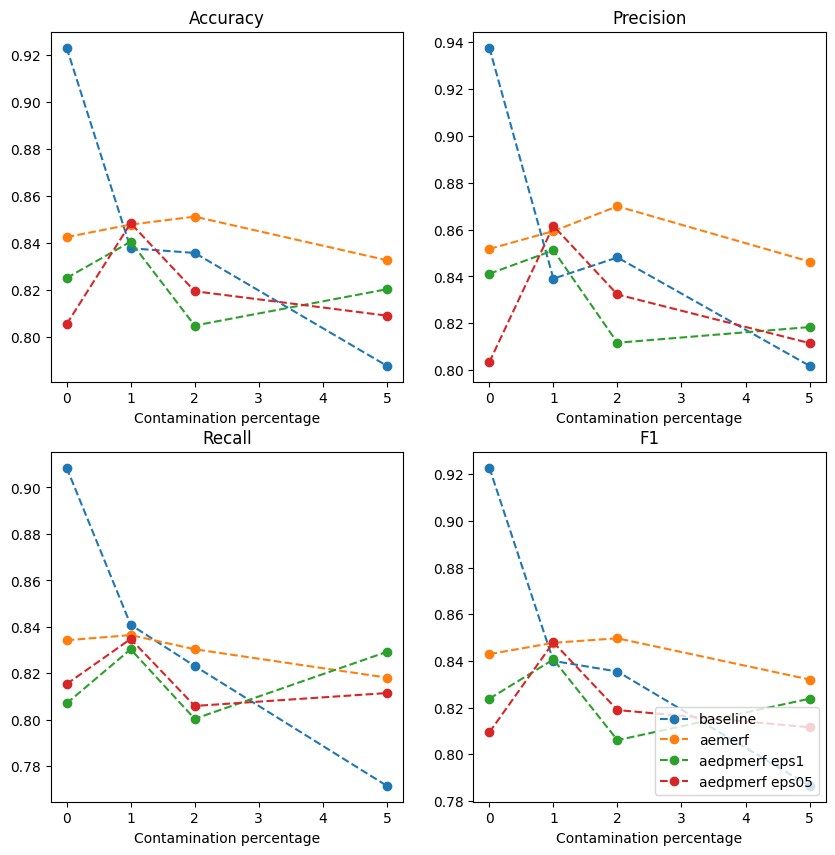
\includegraphics[width=0.8\textheight]{results_aedpmerf_contam.png}}

        \caption{Contaminated training set: AE-(DP)MERF}

    \end{figure}
\end{frame}

